\documentclass{beamer}
\usetheme{Berkeley}
\usecolortheme{seagull}
\usefonttheme{serif}
%\usefonttheme{structuresmallcapsserif} %forse un po' troppo pretenzioso

\usepackage[english,italian]{babel}
\usepackage{lipsum}
\usepackage{siunitx}
\usepackage{tikz}
\usepackage{pgfplots}
\usepackage{pgfplotstable}
\pgfplotsset{
	compat=newest,
	every tick label/.append style={font=\small},
	every node near coord/.append style={font=\small}
}
\usepgfplotslibrary{ternary}
\usetikzlibrary{calc}
%\usepackage{todonotes} %non sembra funzionare con beamer
\usepackage{url}
\usepackage[export]{adjustbox}
\usepackage[font={footnotesize,color=darkgray},justification=centering]{caption}

\title{OpenLDAT}
\subtitle{Un sistema di misurazione di metriche di latenza dei display}
\author{Federico Dossena}
\institute{Università degli Studi di Milano}
\date{2021-??-??}

\begin{document}
	
\begin{frame}
	\titlepage
\end{frame}

\section{Introduzione}
\begin{frame}
	\frametitle{Introduzione}
	\begin{itemize}
		\item Progetto nato dall'esigenza di \textcolor{blue}{misurare la latenza totale di un sistema} in modo automatico
		\item \textcolor{blue}{Nessun dispositivo simile sul mercato}, solitamente si usa un mouse con collegato un LED e una telecamera ad alta velocità
		\item \textcolor{blue}{OpenLDAT può misurarla in modo automatico}, e può fare anche molto altro
		\item Progetto totalmente \textcolor{blue}{libero}
	\end{itemize}
	\begin{block}{Latenza totale del sistema}
		Tempo che intercorre tra un'azione nel mondo fisico, come un click del mouse, e la visualizzazione del risultato sul display.
	\end{block}
\end{frame}
\begin{frame}[shrink=10]
	\frametitle{Nvidia LDAT}
	\begin{columns}
		\column{0.5\textwidth}
		\begin{itemize}
			\item A Settembre 2020, Nvidia ha inviato dei prototipi di \textcolor{blue}{Nvidia LDAT} ad alcuni giornalisti specializzati, ma poi \textcolor{blue}{non ha commercializzato il prodotto}
			\item Il dispositivo permetteva di misurare la \textcolor{blue}{latenza totale del sistema} in modo manuale o semi-automatico
			\item Il progetto \textcolor{blue}{OpenLDAT} vuole ricreare questo dispositivo, aggiungere più funzioni, e utilizzarlo per testare dei display
		\end{itemize}
		\column{0.5\textwidth}
		\begin{figure}
			\centering
			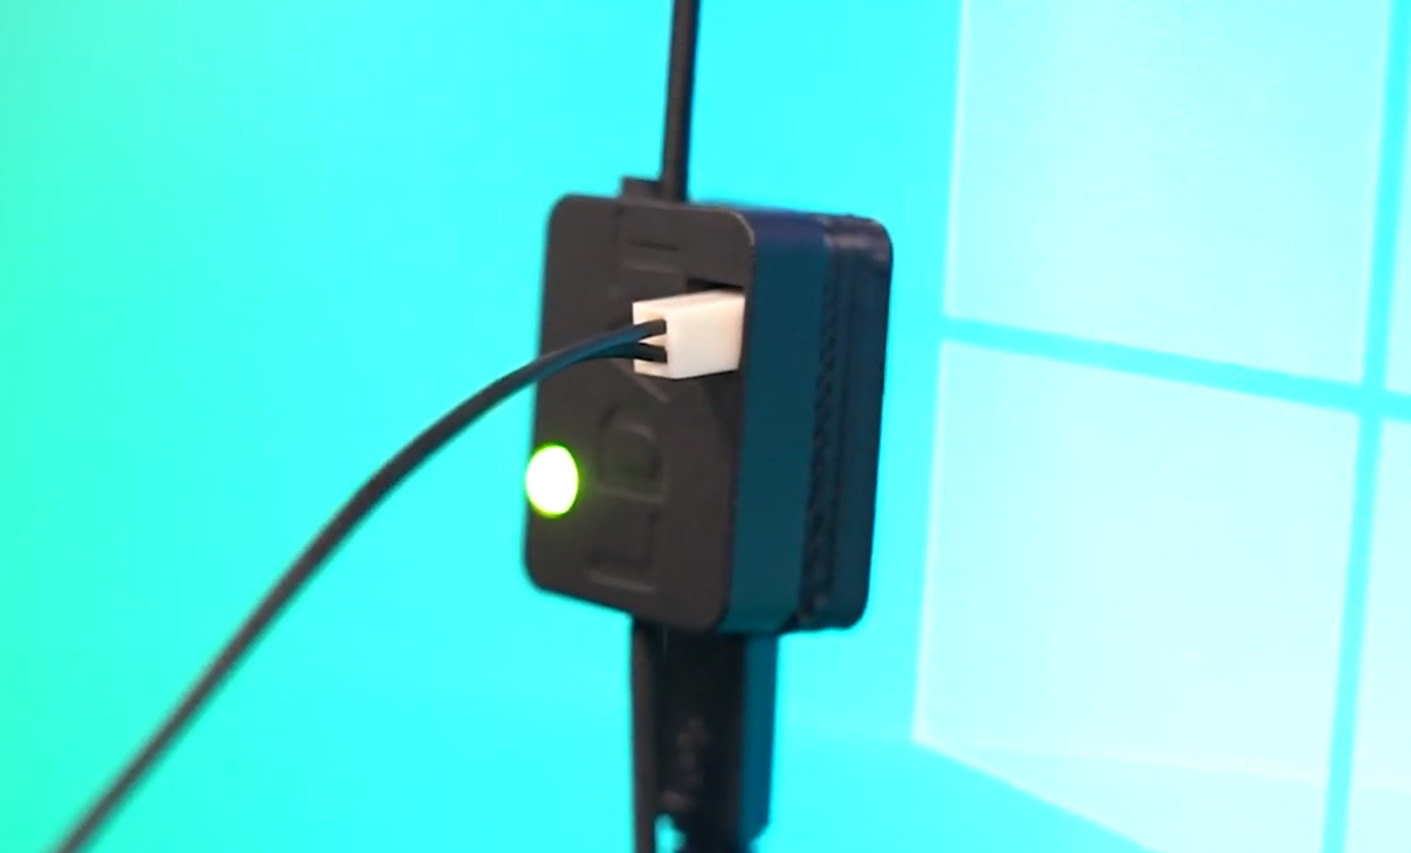
\includegraphics[width=\textwidth]{StatoDellArte_files/nvldat_front.jpg}
			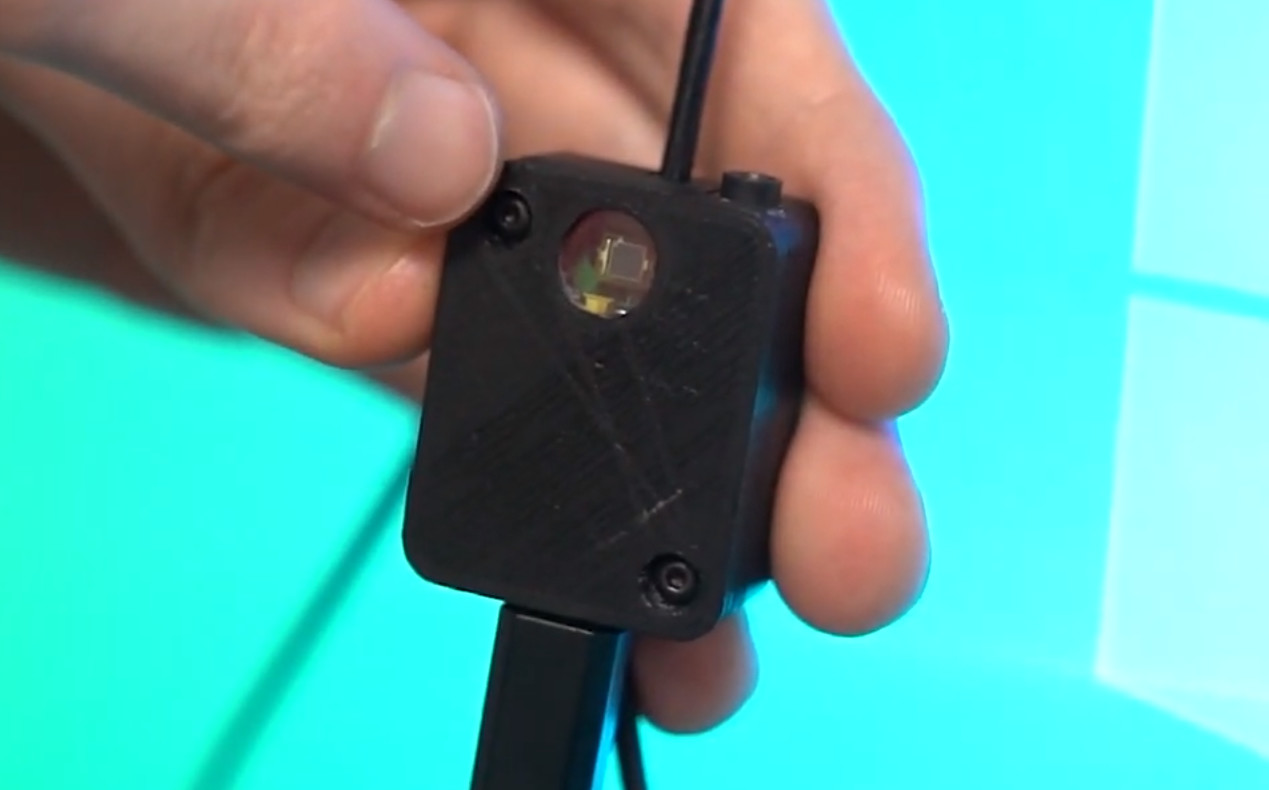
\includegraphics[width=\textwidth]{StatoDellArte_files/nvldat_back.jpg}
			\caption*{Dispositivo Nvidia LDAT}
		\end{figure}
		
	\end{columns}
	
\end{frame}

\section{Dispositivo}
\begin{frame}[shrink=10]
	\frametitle{Dispositivo OpenLDAT (1)}
	\begin{columns}
		\column{0.5\textwidth}
		\begin{itemize}
			\item Microcontroller \textcolor{blue}{ATmega32U4}
			\item Fototransistor \textcolor{blue}{ALS-PT19} con \textcolor{blue}{4 livelli di gain} del sensore controllabili via software
		\end{itemize}
		\column{0.5\textwidth}
		\begin{itemize}
			\item \textcolor{blue}{PCB} personalizzato
			\item Campionamento fino a \textcolor{blue}{\textasciitilde 30kHz 10-bit}
			\item Comunicazione via USB HID e CDC Serial, \textcolor{blue}{nessun driver richiesto}
		\end{itemize}
	\end{columns}
	\begin{figure}
		\centering
		\adjincludegraphics[trim={{.10\width} 0 {.20\width} 0},clip,height=0.55\textheight]{Dispositivo_files/assembly_10.jpg}
		\adjincludegraphics[trim={{.12\width} 0 {.18\width} 0},clip,height=0.55\textheight]{Dispositivo_files/assembly_09.jpg}
		\caption*{Hardware del dispositivo OpenLDAT}
	\end{figure}
\end{frame}
\begin{frame}
	\frametitle{Dispositivo OpenLDAT (2)}
	\begin{columns}
		\column{0.5\textwidth}
		\begin{itemize}
			\item Generazione dei \textcolor{blue}{click automatica o manuale} tramite input esterno
			\item \textcolor{blue}{LED per validazione} con telecamera ad alta velocità
			\item \textcolor{blue}{Case stampabile} in 3D
			\item \textcolor{blue}{Poco costoso e facile da realizzare} anche da un maker
		\end{itemize}
		\column{0.5\textwidth}
		\begin{figure}
			\adjincludegraphics[trim={{.22\width} 0 {.22\width} 0},clip,width=\textwidth]{Dispositivo_files/assembly_15.jpg}
			\caption*{Dispositivo OpenLDAT assemblato}
		\end{figure}
	\end{columns}
\end{frame}

\section{Applicazione}
\begin{frame}[shrink=15]
	\frametitle{Applicazione OpenLDAT (1)}
	\begin{columns}
		\column{0.5\textwidth}
		\begin{itemize}
			\item \textcolor{blue}{Applicazione grafica} Java SE e OpenGL
			\item Permette di \textcolor{blue}{configurare, eseguire i test, e visualizzarne i risultati} in modo semplice
		\end{itemize}
		\column{0.5\textwidth}
		\begin{itemize}
			\item \textcolor{blue}{Esportazione dei dati} per un analisi esterna
			\item \textcolor{blue}{Include un manuale} che spiega i test
			\item \textcolor{blue}{Multipiattaforma} (Windows, GNU/Linux, MacOS)
		\end{itemize}
	\end{columns}
	\begin{figure}
		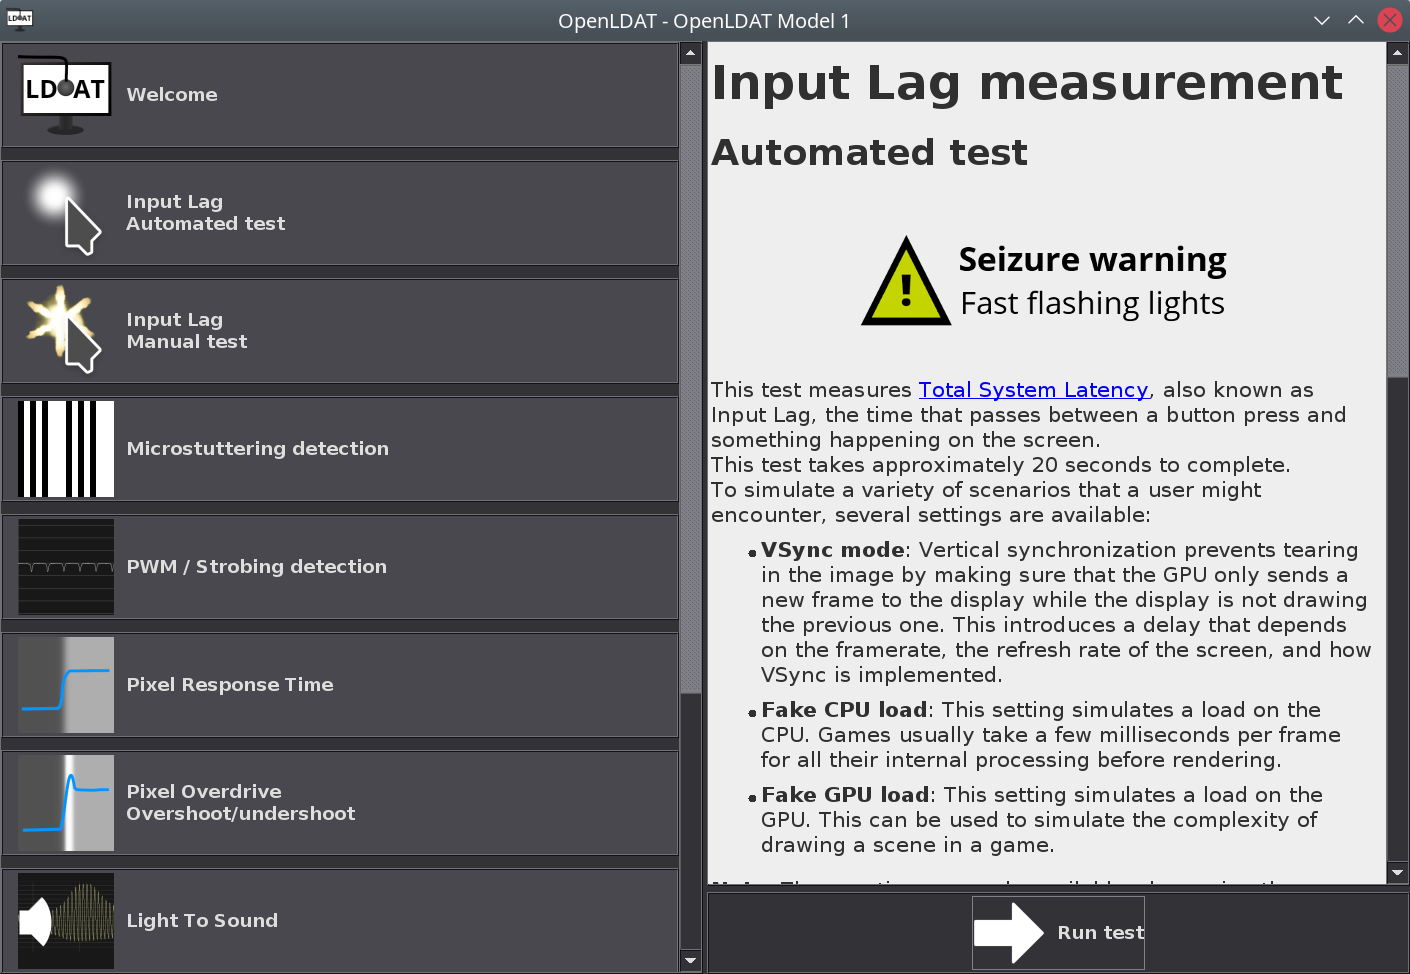
\includegraphics[height=0.7\textheight]{Applicazione_files/gui_mainMenu2.png}
		\caption*{Schermata principale dell'applicazione}
	\end{figure}
\end{frame}
\begin{frame}[shrink=7]
	\frametitle{Applicazione OpenLDAT (2)}
	Elenco dei test:\begin{itemize}
		\item \textcolor{blue}{Latenza totale del sistema}:\begin{itemize}
			\item \textcolor{blue}{Test automatico} con OpenGL e generazione automatica dei click
			\item \textcolor{blue}{Test manuale} utilizzando un'applicazione e la generazione automatica dei click o un mouse/controller modificato
		\end{itemize}
		\item \textcolor{blue}{Rilevamento del microstuttering}: rileva perdita/duplicazione di fotogrammi
		\item \textcolor{blue}{Rilevamento di PWM e noise}: rileva la frequenza del lampeggio della retroilluminazione e altri tipi di noise
		\item \textcolor{blue}{Tempi di risposta dei pixel}: misura il tempo di transizione dei pixel
		\item \textcolor{blue}{Misurazione dell'overdrive}: misura l'errore commesso durante la transizione dei pixel
		\item \textcolor{blue}{Light To Sound}: permette di ascoltare il segnale dal sensore, utile per rilevare fonti di rumore, ma anche per divertimento
	\end{itemize}
\end{frame}
\begin{frame}
	\frametitle{Applicazione OpenLDAT (3)}
	\begin{figure}
		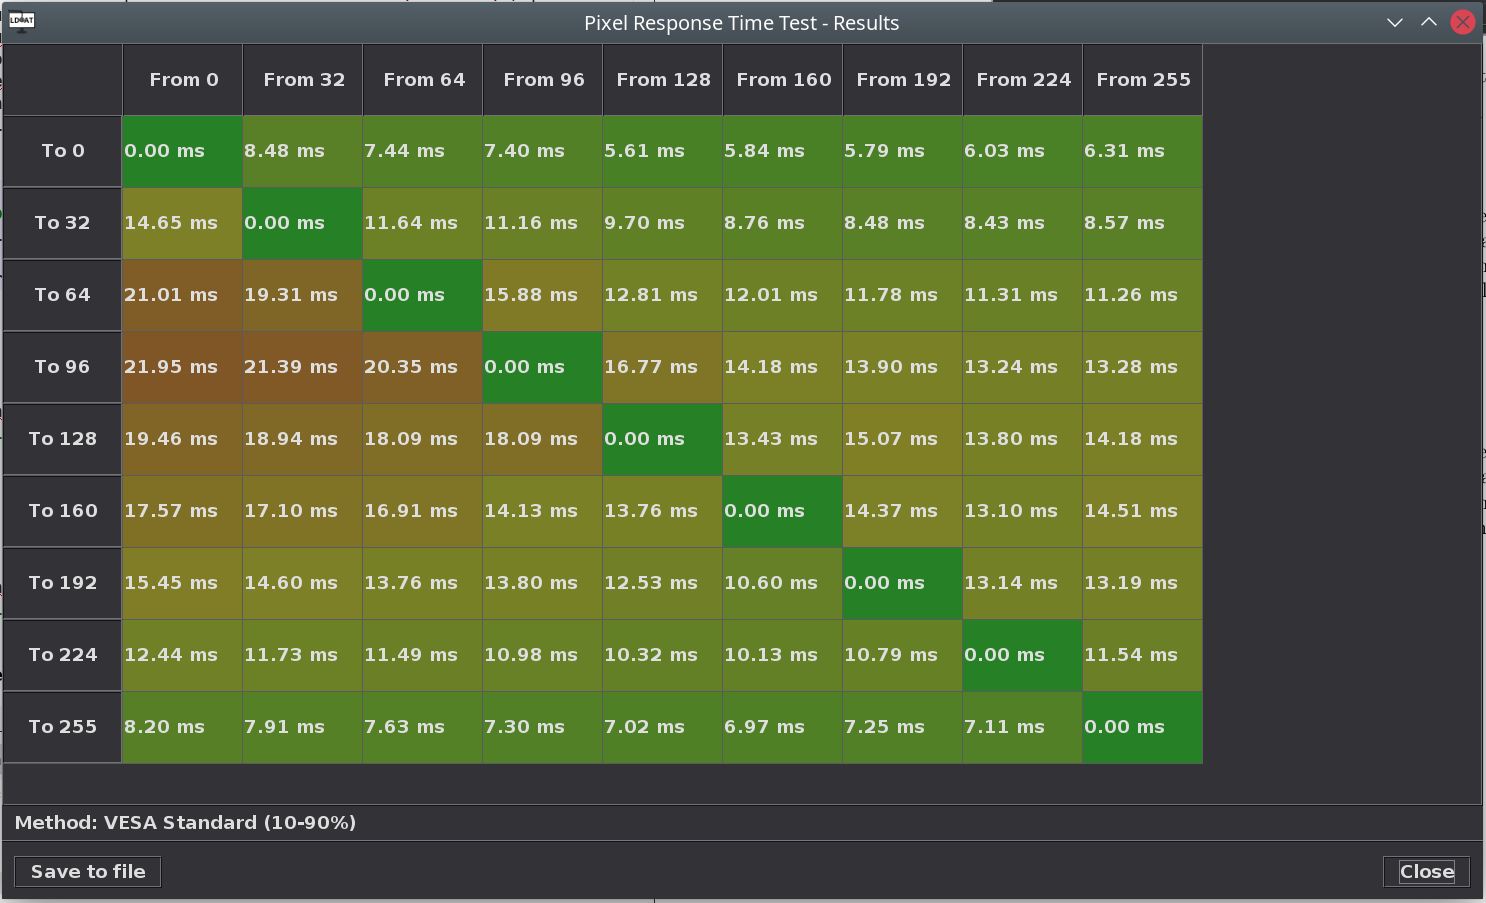
\includegraphics[width=\textwidth]{Applicazione_files/gui_pixelresponse_results.png}
		\caption*{Esempio di risultati di un test dei tempi di risposta dei pixel (AOC Q2770P)}
	\end{figure}
\end{frame}

\section{Risultati sperimentali}
\begin{frame}[shrink=10]
	\frametitle{Risultati sperimentali}
	\textcolor{blue}{Oltre 20 display di tipi e periodi diversi sono stati testati} dall'autore e da terzi che hanno ricevuto un prototipo e istruzioni su come eseguire i test.
	\begin{table}
		\centering
		\resizebox{11cm}{!}{\begin{tabular}{|l|c|c|c|c|c|c|} 
			\hline
			\textbf{Dispositivo} & \textbf{Tipo} & \textbf{Anno} & \textbf{Refresh} & \textbf{Tecnologia} & \textbf{Retroilluminazione} & \textbf{Testato da}  \\ 
			\hline
			Acer Predator XB271HU & Monitor & 2019 & 165Hz VRR & TN  & Edge LED & Terzi \\ \hline
			Acer Swift 3 & Laptop & 2020 & 60Hz & IPS & Edge LED & Autore \\ \hline
			AOC Q2770P & Monitor & 2014 & 60Hz & IPS & Edge LED & Autore \\ \hline
			ASUS VP228HE & Monitor & 2019 & 60Hz & TN & Edge LED & Terzi \\ \hline
			ASUS VW228 & Monitor & 2011 & 60Hz & TN & Edge LED & Terzi \\ \hline
			BenQ GL2706PQ & Monitor & 2014 & 60Hz & TN & Edge LED & Terzi \\ \hline
			BenQ XL2420T & Monitor & 2012 & 120Hz & TN & Edge LED & Terzi \\ \hline
			Huawei MateBook D & Laptop & 2019 & 60Hz & IPS & Edge LED & Terzi \\ \hline
			iPhone 6S & Smartphone & 2015 & 60Hz & IPS & Edge LED & Terzi \\ \hline
			LG 27GL850-B & Monitor & 2018 & 144Hz VRR & IPS HDR & Edge LED & Terzi \\ \hline
			LG E2360 & Monitor & 2012 & 60Hz & TN & Edge LED & Terzi \\ \hline
			MacBook Pro 13" & Laptop & 2017 & 60Hz & IPS & Edge LED & Terzi \\ \hline
			Octigen M19W & Monitor & 2008 & 60Hz & TN & CCFL & Autore \\ \hline
			OnePlus 3T & Smartphone & 2016 & 60Hz & AMOLED & N/A & Autore \\ \hline
			OnePlus 7 Pro & Smartphone & 2019 & 90Hz VRR & AMOLED & N/A & Terzi \\ \hline
			Philips 32PFS4132 & TV & 2020 & 60Hz & TN & Edge LED & Autore \\ \hline
			Philips 105MB & Monitor & 1997 & N/A & CRT & N/A & Autore \\ \hline
			Samsung C34H890 & Monitor & 2019 & 100Hz VRR & VA & LED Array & Terzi \\ \hline
			Samsung P2770HD & TV & 2011 & 60Hz & TN & Edge LED & Autore \\ \hline
			Sony VAIO SVF1532C5E & Laptop & 2014 & 60Hz & TN & Edge LED & Terzi \\ \hline
			Sharp Aquos LC-40FG3242E & TV & 2020 & 60Hz & TN & Edge LED & Autore \\ \hline
			Thinkpad T480 & Laptop & 2018 & 60Hz & IPS & Edge LED & Autore \\ \hline
		\end{tabular}}
		\caption*{Lista completa dei dispositivi testati}
	\end{table}
\end{frame}
\begin{frame}[fragile,shrink=40]
	\frametitle{Input lag (1)}
	\begin{figure}
		\pgfplotstableread[col sep=comma]{
			model,novsync,vsync
			Acer Predator XB271HU (165Hz G-Sync),6.3,32.5
			LG 27GL850-B (144Hz Freesync),6.4,36.9
			BenQ XL2420T (120Hz),9.2,44.1
			%Huawei Matebook D 2019 (60Hz Laptop),10.1,86.3 %dubito dell'accuratezza di questo risultato, sembra troppo basso il vsync off, probabilmente il tizio si è mosso durante il test
			Samsung C34H890 (100Hz Freesync),11.8,52.8
			Philips 105MB (85Hz CRT),13.1,64.2
			ASUS VP228HE (60Hz),13.1,86.8
			LG E2360 (60Hz),14.1,89.6
			Sony VAIO SVF1532C5E (60Hz Laptop),15.5,62.4
			ASUS VW228 (60Hz),16.0,88.5
			Thinkpad T480 2018 (60Hz Laptop),18.2,88.8
			Octigen M19W (60Hz),19.6,88.2
			BenQ GL2706PQ (60Hz),27.7,93.7
			AOC Q2770P (60Hz),29.8,95.8
			MacBook Pro 13" 2017 (60Hz Laptop),30.2,96.7
			Acer Swift 3 (60Hz Laptop),31.8,111.2
			Philips 32PFS4132 (60Hz TV),34.9,106.5
			Sharp LC-40FG3242E (60Hz TV),37.1,108.8
			Samsung P2770HD (60Hz TV),41.1,111.9
		}\dataset
		\begin{tikzpicture}
			\begin{axis}[xbar, bar width=8pt, y dir=reverse, ytick=data, yticklabels from table={\dataset}{model}, yticklabel style={text width=6cm, align=right}, table/y expr = \coordindex, nodes near coords, reverse legend, xlabel=Ritardo (ms), width=19cm, height=17.5cm, xmin=0, ymin=-1, ymax=18] %ymax messo a mano con il numero di display per migliore formattazione
				\addplot table[x=vsync] {\dataset};
				\addplot table[x=novsync] {\dataset};
				\legend{VSync On, VSync Off}
			\end{axis}
		\end{tikzpicture}
		%\caption*{Input lag dei display testati}
	\end{figure}
\end{frame}
\begin{frame}[fragile,shrink=35]
	\frametitle{Input lag (2)}
	\begin{figure}
		\pgfplotstableread[col sep=comma]{
			app,lag,emin,emax
			Mass Effect Legendary Ed. (2021),45.7,8.4,7.7
			Crysis (2007),51.9,6.7,8.6
			Doom Eternal (2020),52.8,4.6,2.4
			Unreal Tournament 2004 (2003),81.3,11.8,18.7
			Google Stadia 1080p60 (FTTH),121.4,34.4,119.6
			YouTube (Chromium),147.2,13.0,17.2
			Doom (1993),158.9,16.9,14.2
			Crysis Remastered (2020),182.5,17.8,23.5
		}\dataset
		\begin{tikzpicture}
			\begin{axis}[xbar, bar width=10pt, y dir=reverse, ytick=data, yticklabels from table={\dataset}{app}, yticklabel style={text width=5.5cm, align=right}, table/y expr = \coordindex, nodes near coords, xlabel=Ritardo (ms), width=11cm, height=8cm, ymin=-1, ymax=8] %ymax messo a mano con il numero di test per migliore formattazione
				\addplot[fill=gray, error bars/.cd, x dir = both, x explicit] table[x=lag, x error plus=emax, x error minus=emin] {\dataset};
			\end{axis}
		\end{tikzpicture}
		%\caption*{Input lag di alcune applicazioni. (150ms è generalmente considerato il limite accettabile per un videogioco)}
	\end{figure}
	\begin{figure}
		\pgfplotstableread[col sep=comma]{
			config,novsync,vsync
			Linux + AMD,28.7,86.1
			Linux + Nvidia (Proprietary),28.0,69.1
			Linux + Nvidia (Nouveau),44.3,86.0
			Linux + Intel,34.1,86.6
			Windows + AMD,29.6,93.9
			Windows + Nvidia,28.4,95.3
			Windows + Intel,31.3,103.4
		}\dataset
		\begin{tikzpicture}
			\begin{axis}[xbar, bar width=8pt, y dir=reverse, ytick=data, yticklabels from table={\dataset}{config}, yticklabel style={text width=5cm, align=right}, table/y expr = \coordindex, nodes near coords, reverse legend, legend style={at={(13.5cm,0.5)},anchor=east}, xlabel=Ritardo (ms), width=12cm, height=8cm, ymin=-1, ymax=7,xmax=120]
				\addplot table[x=vsync] {\dataset};
				\addplot table[x=novsync] {\dataset};
				\legend{VSync On, VSync Off}
			\end{axis}
		\end{tikzpicture}
		%\caption*{Input lag con combinazioni hardware/software diverse}
	\end{figure}
\end{frame}
\begin{frame}
	\frametitle{PWM e noise}
	\begin{table}
		\centering
		\resizebox{8cm}{!}{\begin{tabular}{|l|c|c|} 
			\hline
			\textbf{Dispositivo} & \textbf{Frequenza PWM} & \textbf{Refresh rilevabile}  \\ 
			\hline
			Acer Predator XB271HU & No & No \\ \hline
			Acer Swift 3 & No & No \\ \hline
			AOC Q2770P & No & No \\ \hline
			ASUS VP228HE & No & Si \\ \hline
			ASUS VW228 & 240Hz & No \\ \hline
			BenQ GL2706PQ & No & Si \\ \hline
			BenQ XL2420T & No & No \\ \hline
			Huawei MateBook D 2019 & No & No \\ \hline
			iPhone 6S & No & No \\ \hline
			LG 27GL850-B & No & No \\ \hline
			LG E2360 & 240Hz & No \\ \hline
			MacBook Pro 13" 2017 & No & No \\ \hline
			Octigen M19W & N/A (CCFL) & No \\ \hline
			OnePlus 3T & 240Hz & Si \\ \hline
			OnePlus 7 Pro & No & Si \\ \hline
			Philips 32PFS4132 & 150Hz & No \\ \hline
			Philips 105MB & N/A (CRT) & Si \\ \hline
			Samsung C34H890 & No & Si \\ \hline
			Samsung P2770HD & 180Hz & No \\ \hline
			Sony VAIO SVF1532C5E & No & No \\ \hline
			Sharp Aquos LC-40FG3242E & 180Hz & No \\ \hline
			Thinkpad T480 2018 & No & No \\ \hline
		\end{tabular}}
		%\caption*{PWM e noise dei display testati}
	\end{table}
\end{frame}
\begin{frame}[fragile,shrink=40]
	\frametitle{Risposta dei pixel}
	\begin{figure}
		\centering
		\pgfplotstableread[col sep=comma]{
			model,odoff,odoffemin,odoffemax,odon,odonemin,odonemax,fix
			BenQ XL2420T (TN),NaN,NaN,NaN,2.61,1.48,3.80,-10
			Acer Predator XB271HU (TN),NaN,NaN,NaN,4.06,2.79,3.76,-10
			ASUS VP228HE (TN),4.80,3.39,11.83,NaN,NaN,NaN,-10
			Samsung C34H890 (VA),7.81,5.17,27.90,7.79,4.26,18.25,-10
			Sharp Aquos LC-40FG3242E (TN),NaN,NaN,NaN,8.44,5.71,20.67,-10
			Philips 32PFS4132 (TN),NaN,NaN,NaN,9.38,2.84,3.61,-10
			LG 27GL850-B (IPS HDR),9.74,3.94,4.46,2.91,1.92,11.69,-10
			AOC Q2770P (IPS),12.33,6.06,9.01,7.37,3.09,3.74,-10
			BenQ GL2706PQ (TN),12.97,11.60,9.08,2.59,1.41,3.72,-10
			ASUS VW228 (TN),13.13,12.09,29.60,NaN,NaN,NaN,-10
			Samsung P2770HD (TN),13.34,10.70,17.19,NaN,NaN,NaN,-10
			LG E2360 (TN),13.98,12.36,29.25,NaN,NaN,NaN,-10
			Octigen M19W (TN),14.61,13.10,13.03,NaN,NaN,NaN,-10
			Acer Swift 3 (IPS),15.01,5.04,10.21,NaN,NaN,NaN,-10
			Thinkpad T480 2018 (IPS),15.76,6.01,7.18,NaN,NaN,NaN,-10
			Huawei MateBook D 2019 (IPS),16.98,4.05,14.31,NaN,NaN,NaN,-10
			Sony VAIO SVF1532C5E (TN),17.50,14.39,16.04,NaN,NaN,NaN,-10
			MacBook Pro 13" 2017 (IPS),19.49,8.74,12.60,NaN,NaN,NaN,-10
		}\dataset
		\begin{tikzpicture}
			\begin{axis}[xbar, bar width=8pt, y dir=reverse, ytick=data, yticklabels from table={\dataset}{model}, yticklabel style={text width=5cm, align=right}, table/y expr = \coordindex, nodes near coords, reverse legend, xlabel=Tempo di risposta (ms), width=18cm, height=16.5cm, xmin=0, ymin=-1, ymax=18] %ymax messo a mano con il numero di display per migliore formattazione
				\addplot plot[forget plot] table[x=fix] {\dataset};
				\addplot plot [error bars/.cd, x dir = both, x explicit] table[x=odoff, x error plus=odoffemax, x error minus=odoffemin] {\dataset};
				\addplot plot [error bars/.cd, x dir = both, x explicit] table[x=odon, x error plus=odonemax, x error minus=odonemin] {\dataset};
				\legend{Overdrive Off, Overdrive On}
			\end{axis}
		\end{tikzpicture}
		%\caption*{Tempi di riposta dei display testati}
	\end{figure}
\end{frame}
\begin{frame}[fragile,shrink=40]
	\frametitle{Overdrive}
	\begin{figure}[h!]
		\centering
		\pgfplotstableread[col sep=comma]{
			model,odoff,odoffemin,odoffemax,odon,odonemin,odonemax,fix
			BenQ XL2420T (TN),NaN,NaN,NaN,2.80,2.56,14.55,-10
			Acer Predator XB271HU (TN),NaN,NaN,NaN,7.90,7.26,14.81,-10
			Samsung C34H890 (VA),0.32,0.32,1.79,1.21,1.21,6.43,-10
			LG 27GL850-B (IPS HDR),0.39,0.39,0.22,26.39,24.82,22.98,-10
			AOC Q2770P (IPS),0.17,0.17,0.41,4.14,4.14,16.32,-10
			BenQ GL2706PQ (TN),0.56,0.35,0.82,11.75,9.87,33.99,-10
			ASUS VP228HE (TN),0.44,0.44,1.14,NaN,NaN,NaN,-10
			Octigen M19W (TN),0.25,0.25,0.65,NaN,NaN,NaN,-10
			Acer Swift 3 (IPS),0.35,0.35,0.25,NaN,NaN,NaN,-10
			Thinkpad T480 2018 (IPS),0.17,0.17,0.36,NaN,NaN,NaN,-10
			Huawei MateBook D 2019 (IPS),0.15,0.15,0.31,NaN,NaN,NaN,-10
			Sony VAIO SVF1532C5E (TN),0.31,0.21,0.93,NaN,NaN,NaN,-10
			MacBook Pro 13" 2017 (IPS),0.22,0.22,0.59,NaN,NaN,NaN,-10
		}\dataset
		\begin{tikzpicture}
			\begin{axis}[xbar, bar width=8pt, y dir=reverse, ytick=data, yticklabels from table={\dataset}{model}, yticklabel style={text width=5cm, align=right}, table/y expr = \coordindex, nodes near coords, reverse legend, xlabel=Errore di transizione (\%), width=13cm, height=13cm, xmin=0, ymin=-1, ymax=13] %ymax messo a mano con il numero di display per migliore formattazione]
				\addplot plot[forget plot] table[x=fix] {\dataset};
				\addplot plot [error bars/.cd, x dir = both, x explicit] table[x=odoff, x error plus=odoffemax, x error minus=odoffemin] {\dataset};
				\addplot plot [error bars/.cd, x dir = both, x explicit] table[x=odon, x error plus=odonemax, x error minus=odonemin] {\dataset};
				\legend{Overdrive Off, Overdrive On}
			\end{axis}
		\end{tikzpicture}
		%\caption*{Errore di transizione in percentuale assoluta. Sono omessi gli schermi con retroilluminazione PWM}
	\end{figure}
\end{frame}
\begin{frame}
	\frametitle{Microstuttering}
	\begin{table}[h!]
		\centering
		\resizebox{8cm}{!}{\begin{tabular}{|l|c|c|} 
			\hline
			\textbf{Dispositivo} & \textbf{Refresh nativo} & \textbf{Overclock}  \\ 
			\hline
			Acer Predator XB271HU & No & No \\ \hline
			Acer Swift 3 & No & N/A \\ \hline
			AOC Q2770P & No & Si \\ \hline
			ASUS VP228HE & No & No \\ \hline
			ASUS VW228 & No & N/A \\ \hline
			BenQ GL2706PQ & No & Si \\ \hline
			BenQ XL2420T & No & No \\ \hline
			Huawei MateBook D 2019 & No & N/A \\ \hline
			LG 27GL850-B & No & No \\ \hline
			LG E2360 & No & No \\ \hline
			Octigen M19W & No & No \\ \hline
			Philips 32PFS4132 & No & N/A \\ \hline
			Philips 105MB & No & No \\ \hline
			Samsung C34H890 & No & No \\ \hline
			Samsung P2770HD & No & N/A \\ \hline
			Sony VAIO SVF1532C5E & No & N/A \\ \hline
			Sharp Aquos LC-40FG3242E & No & N/A \\ \hline
			Thinkpad T480 2018 & No & N/A \\ \hline
		\end{tabular}}
		%\caption*{Confronto della presenza di \textit{microstuttering} tra i display testati. N/A indica che non è stato possibile eseguire l'\textit{overclock} su questo dispositivo}
	\end{table}
\end{frame}

\section{Conclusioni}
\begin{frame}
	\frametitle{Conclusioni}
	\lipsum[1]
\end{frame}
\begin{frame}
	\frametitle{Grazie per l'attenzione}
	\centering
	Per maggiori informazioni:
	\textcolor{blue}{\url{https://openldat.fdossena.com}}
\end{frame}

\end{document}
